 \setlength{\baselineskip}{20pt}
\chapter{多帧时序特征融合的停车位检测方法}
\label{cha:chap4}



\section{研究动机}
在真实停车场景中，环视相机采集的连续帧图像存在明显的时序相关性。尽管单帧结构感知检测方法能够在静态图像条件下有效提升停车位检测的结构一致性，但在真实驾驶与泊车过程中，车辆获取的是连续帧视觉信息。受视角变化、动态遮挡以及环境噪声等因素影响（停车位位置在相邻帧中基本稳定，仅光照、阴影、遮挡略有变化，而噪声、反射或标线模糊在单帧中可能导致检测不稳定），现有方法仅基于单帧特征进行检测，忽略了时序上下文信息，导致在动态场景（光照闪烁、行人经过等）下精度波动。

从任务本质上看，停车位检测并非完全静态的问题，而是具有明显的时序属性。相邻帧之间在空间结构和语义信息上具有高度相关性，合理利用时序信息有助于弥补单帧检测在复杂场景中的不确定性。然而，现有研究中对停车位检测时序建模的关注仍相对有限，如何在保持端到端检测流程的同时，引入有效的时序特征融合机制，仍有待进一步探索。

本章在单帧结构感知检测方法的基础上，进一步将停车位检测问题从静态图像建模扩展至多帧时序建模。通过对连续帧中结构感知表示进行时序特征融合，显式建模停车位在时间维度上的一致性，有效缓解了单帧检测中由遮挡与视角变化引起的不稳定问题。该方法从建模维度上实现了由空间结构感知向时空联合感知的扩展，使停车位检测更加贴近真实驾驶场景。




\section{方法介绍}
如图\ref{fig_pip3}所示，多帧时序特征融合的停车位检测方法在单帧结构感知检测框架的基础上，引入了跨时帧自注意力机制和时序一致性约束，实现了时空联合感知的停车位检测。

\begin{figure}[!h]
\centering
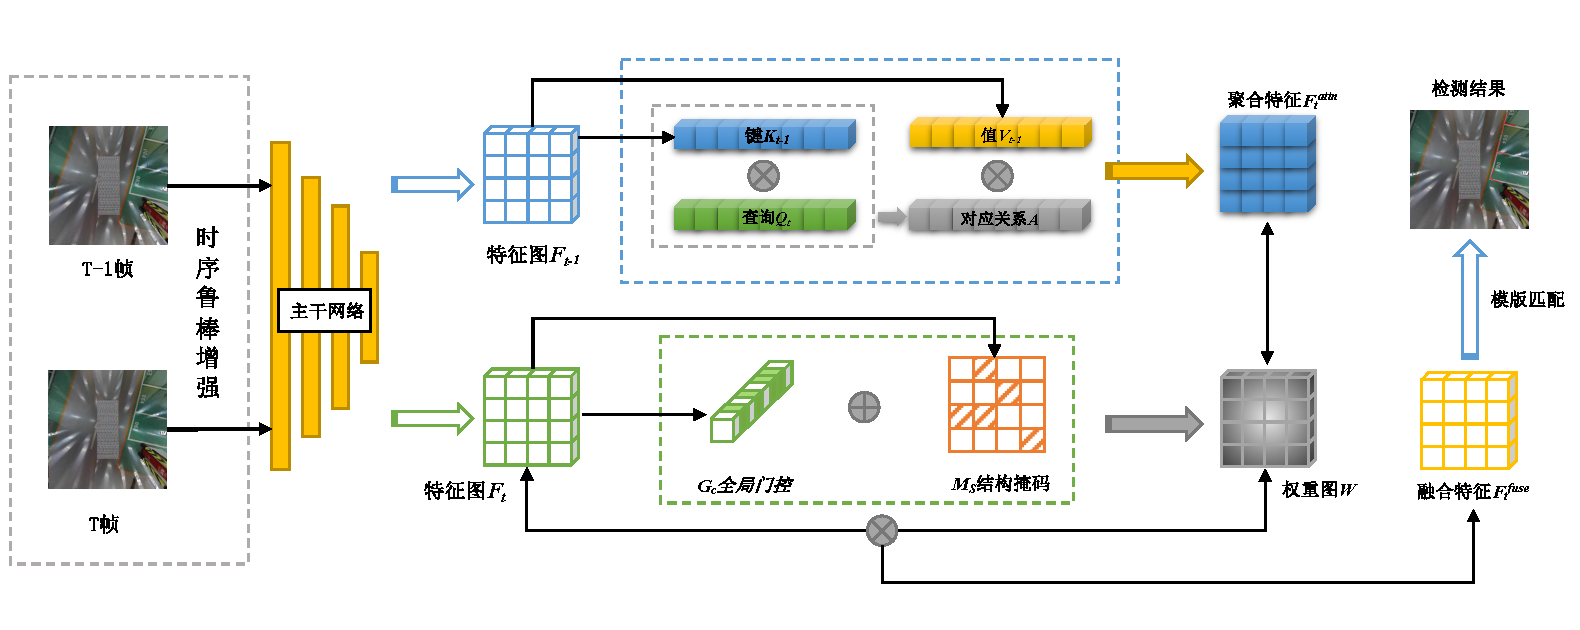
\includegraphics[width=1\textwidth]{figures/chp4/pipline_3.pdf}
\caption{多帧时序特征融合的停车位检测框架示意图 \\Fig~\ref{fig_pip3}~Overview of parking space detection method based on multi-frame temporal feature fusion}
\label{fig_pip3}
\end{figure}

\subsection{跨时帧自注意力}

在自动泊车场景中，相邻视频帧之间具有较强的时序连续性，停车位的几何结构与空间布局在短时间内基本保持稳定。为充分利用这一时序先验信息，本文提出跨帧自注意力机制，用于在特征层面实现多帧时序信息的自适应融合，增强当前帧对停车位结构的表征能力。

设当前帧与前一帧提取的特征分别为
$\mathbf{F}_t \in \mathbb{R}^{B \times C \times H \times W}, \quad
\mathbf{F}_{t-1} \in \mathbb{R}^{B \times C \times H \times W}$,
其中 B 表示批量大小，C 为通道数，H 与 W 为空间分辨率。跨帧自注意力模块以当前帧特征作为查询项，以前一帧特征作为键和值，通过注意力机制显式建模两帧之间的空间关联关系。

首先，采用 $1\times1$ 卷积对输入特征进行线性映射，分别生成查询（Query）、键（Key）和值（Value）：
$\mathbf{Q} = \phi_q(\mathbf{F}_t), \quad
\mathbf{K} = \phi_k(\mathbf{F}_{t-1}), \quad
\mathbf{V} = \phi_v(\mathbf{F}_{t-1})$,
其中 $\phi_q(\cdot)$、$\phi_k(\cdot)$ 和 $\phi_v(\cdot)$ 表示可学习的线性投影。为提升模型对不同语义子空间的建模能力，将通道维度划分为 N 个注意力头，并将空间维度展开为 HW，得到：
$\mathbf{Q}, \mathbf{K}, \mathbf{V} \in \mathbb{R}^{B \times N \times \frac{C}{N} \times HW}$.


在每一个注意力头中，采用缩放点积注意力计算当前帧与前一帧之间的相关性：
\begin{equation}
\mathbf{A} = \mathrm{Softmax}(\frac{\mathbf{Q}\mathbf{K}^{\top}}{\sqrt{C/N}}),
\end{equation}

其中 $\mathbf{A}$ 表示当前帧中每一个空间位置对前一帧各位置的注意力权重。该权重刻画了跨帧特征在空间维度上的对应关系，使模型能够自适应地关注历史帧中与当前帧最相关的区域。

基于计算得到的注意力权重，对前一帧的值特征进行加权求和，实现跨帧信息的聚合：
\begin{equation}
\mathbf{F}_{t}^{\mathrm{attn}} = \mathbf{A} \cdot \mathbf{V}
\end{equation}
随后，将多头特征在通道维度上进行拼接，并恢复为原始空间结构，得到融合后的特征表示:
\begin{equation}
\mathbf{F}_{t}^{\mathrm{attn}} \in \mathbb{R}^{B \times C \times H \times W}.
\end{equation}
最后，通过一个 $1\times1$ 卷积对融合特征进行线性变换，进一步整合跨帧信息并增强特征表达能力。

通过上述跨帧自注意力机制，模型能够在特征层面充分利用时序上下文信息，在当前帧特征受遮挡、光照变化或噪声干扰的情况下，仍可从历史帧中补充稳定可靠的停车位结构信息，从而提升停车位检测在复杂场景下的鲁棒性与时序一致性。


\subsection{动态时序融合}
在跨帧自注意力模块中，模型已能够从历史帧中提取与当前帧高度相关的时序信息。然而，不同场景下当前帧与历史帧的可靠性并不一致：在结构清晰、无遮挡的情况下，当前帧特征更具判别性；而在光照突变、遮挡或噪声干扰较强的场景中，历史帧特征往往更加稳定。若对两者进行静态或固定比例的融合，容易引入冗余信息甚至错误引导。

为此，本文进一步提出动态结构感知的时序融合模块，通过联合建模全局通道重要性与局部结构显著性，自适应地调节当前帧特征与跨帧注意力特征之间的融合权重，实现更加稳健的多帧特征整合。

设当前帧特征为
$\mathbf{F}_t \in \mathbb{R}^{B \times C \times H \times W}$,
跨帧自注意力模块输出的历史帧增强特征为
$\mathbf{F}_{t}^{\text{attn}} \in \mathbb{R}^{B \times C \times H \times W}$.
动态融合模块首先从当前帧特征中提取全局通道权重，用以刻画不同语义通道在当前时刻的重要程度。具体而言，通过全局平均池化将空间信息压缩为通道描述向量：
$\mathbf{g} = \text{GAP}(\mathbf{F}_t)$,
并经由 $1\times1$ 卷积与 Sigmoid 函数得到通道级门控权重：
\begin{equation}
\mathbf{G}_c = \sigma\!\left( W_c \mathbf{g} \right),
\quad
\mathbf{G}_c \in \mathbb{R}^{B \times C \times 1 \times 1}
\end{equation}
该权重反映了不同通道在当前帧中的全局响应强度，有助于抑制低置信度语义特征。

与此同时，为突出停车位结构相关的空间区域，模块进一步从当前帧特征中预测结构感知掩码。该掩码通过一组卷积操作生成：
\begin{equation}
\mathbf{M}_s = \sigma\!\left( W_2 \, \delta \!\left( \text{BN}( W_1 * \mathbf{F}_t ) \right) \right),
\quad
\mathbf{M}_s \in \mathbb{R}^{B \times 1 \times H \times W}
\end{equation}
其中 $*$ 表示卷积操作，$\delta(\cdot)$ 为 ReLU 激活函数，$\mathbf{M}_s$ 表示空间维度上的结构显著性权重。该掩码能够自适应地关注停车位边线、角点等关键结构区域，同时弱化背景区域对时序融合的干扰。

随后，将通道级权重与空间结构掩码进行联合建模，通过广播机制得到最终的动态融合权重：
\begin{equation}
\mathbf{W} = \mathbf{G}_c \odot \mathbf{M}_s,
\quad
\mathbf{W} \in \mathbb{R}^{B \times C \times H \times W},
\end{equation}

其中 $\odot$ 表示逐元素乘法。基于该动态权重，当前帧特征与历史帧增强特征按照如下方式进行融合：
\begin{equation}
\mathbf{F}_{t}^{\mathrm{fuse}} =
\mathbf{W} \odot \mathbf{F}_{t}^{\text{attn}}
+ \left( 1 - \mathbf{W} \right) \odot \mathbf{F}_t.
\end{equation}

通过这种动态融合方式，模型能够根据当前场景的结构清晰度和稳定性，自适应地平衡历史信息与当前信息的贡献。在结构清晰的区域，模型更多依赖当前帧特征；在结构模糊或受干扰的区域，则更多参考历史帧的稳定信息，从而实现更稳健的时序特征融合。

上述融合策略使模型能够在空间和通道两个层面上自适应地平衡当前帧与历史帧信息：在结构显著且语义稳定的区域，更倾向于引入跨帧增强特征；而在当前帧信息可靠的区域，则保留更多当前帧特征，从而避免时序信息的过度引入。
通过引入该动态结构感知时序融合模块，模型不仅提升了多帧特征融合的灵活性，还显著增强了在复杂场景下停车位检测的鲁棒性，为后续关键点检测与结构匹配提供了更加稳定且一致的特征表示。




\subsection{时序鲁棒增强}
在多帧时序停车位检测任务中，模型不仅需要学习跨帧特征之间的关联关系，还需要具备对真实驾驶场景中复杂扰动的鲁棒性。在实际应用中，相邻帧之间往往存在亮度变化、噪声干扰、运动模糊以及局部遮挡等非理想因素，若训练阶段未显式考虑这些时序扰动，模型容易对帧间细微变化产生过拟合，从而削弱时序融合模块的有效性。

为此，本文提出时序鲁棒增强策略，在不改变停车位关键点空间坐标的前提下，对相邻帧施加具有物理合理性的图像扰动，模拟真实视频序列中的帧间差异，引导模型学习更加稳健的时序特征表示。该策略在训练阶段对前一帧与当前帧图像进行联合与差异化增强，同时严格保证几何一致性，避免对关键点标注产生破坏。

设前一帧与当前帧原始图像分别为
$\mathbf{I}_{t-1} (\mathbf{I}_t \in \mathbb{R}^{H \times W \times 3})$,
对应的停车位关键点标注为
$\mathcal{P}_t = \{ \mathbf{p}_i \}_{i=1}^{N}$.
时序鲁棒增强的核心原则是在增强过程中保持关键点坐标不变，即增强操作满足：
\begin{equation}
\mathcal{T}(\mathbf{p}_i) = \mathbf{p}_i
\end{equation}
从而保证监督信号在空间上的一致性。

在此约束下，本文首先对相邻帧施加同步光度增强，以模拟环境光照在短时间内的整体变化。具体而言，对两帧图像同时进行亮度与对比度扰动以及轻微高斯模糊处理：
\begin{equation}
\mathbf{I}'_{t-1} = \mathcal{A}_{\text{sync}}(\mathbf{I}_{t-1}), \quad
\mathbf{I}'_{t} = \mathcal{A}_{\text{sync}}(\mathbf{I}_{t})
\end{equation}
该操作保持帧间一致性，有助于模型学习对全局光照变化的不变性。

随后，为模拟真实视频中由曝光变化、传感器噪声或运动引起的帧间差异，仅对当前帧施加非同步光度与退化增强：
\begin{equation}
\tilde{\mathbf{I}}_{t} = \mathcal{A}_{\text{diff}}(\mathbf{I}'_{t}),
\end{equation}
其中 $\mathcal{A}_{\text{diff}}(\cdot)$ 包括亮度与对比度微扰、加性高斯噪声、方向性运动模糊以及 JPEG 压缩伪影等操作。该设计刻意引入前后帧之间的视觉差异，从而逼迫模型在时序融合过程中学会区分结构性信息与瞬时噪声。

此外，为增强模型在遮挡场景下的鲁棒性，本文在当前帧中进一步引入局部随机遮挡增强，通过在随机位置生成若干矩形遮挡区域：
\begin{equation}
\tilde{\mathbf{I}}_{t}(x, y) =
\begin{cases}
\mathbf{r}, & (x,y) \in \Omega_{\text{occ}} \\
\tilde{\mathbf{I}}_{t}(x, y), & \text{otherwise}
\end{cases}
\end{equation}
其中 $\Omega_{\text{occ}}$ 表示遮挡区域，$\mathbf{r}$ 为随机颜色值。该操作模拟车辆、行人或环境物体对停车位边线的局部遮挡，有助于模型利用时序上下文补偿缺失信息。

最后，对当前帧施加轻微的颜色扰动，以 HSV 空间中的饱和度与色调变化形式体现，从而进一步模拟复杂环境下的成像差异。经过上述增强处理后，得到最终用于训练的时序输入对：
\begin{equation}
(\hat{\mathbf{I}}_{t-1}, \hat{\mathbf{I}}_{t}, \mathcal{P}_t)
\end{equation}
其中关键点标注 $\mathcal{P}_t$ 在整个增强过程中保持不变。

通过引入该时序鲁棒增强策略，模型在训练阶段能够充分暴露于多种合理的帧间扰动情形，从而在推理阶段更加依赖结构一致性与时序上下文信息，而非单帧的局部外观特征。这一策略与跨帧自注意力模块及动态结构感知融合模块形成互补，有效提升了多帧停车位检测方法在复杂真实场景下的泛化能力与稳定性。


\section{实验结果及分析}

\subsection{时序数据集PSTD}

为系统评估所提多帧时序停车位检测方法在连续场景下的性能，本文基于CRPS-D数据集构建了专用于时序建模的连续帧数据集，命名为PSTD。CRPS-D是面向复杂真实场景的大规模停车位关键点检测数据集，覆盖多种光照条件、天气环境及停车位布局形式，具有停车位密度高、结构多样性强等特点，能够充分反映实际自动泊车场景中的挑战性因素。PSTD数据集从CRPS-D中筛选并整理具有明确时间连续关系的图像序列，重点用于验证跨帧特征建模与时序鲁棒增强策略的有效性。
\begin{figure}[!h]
\centering
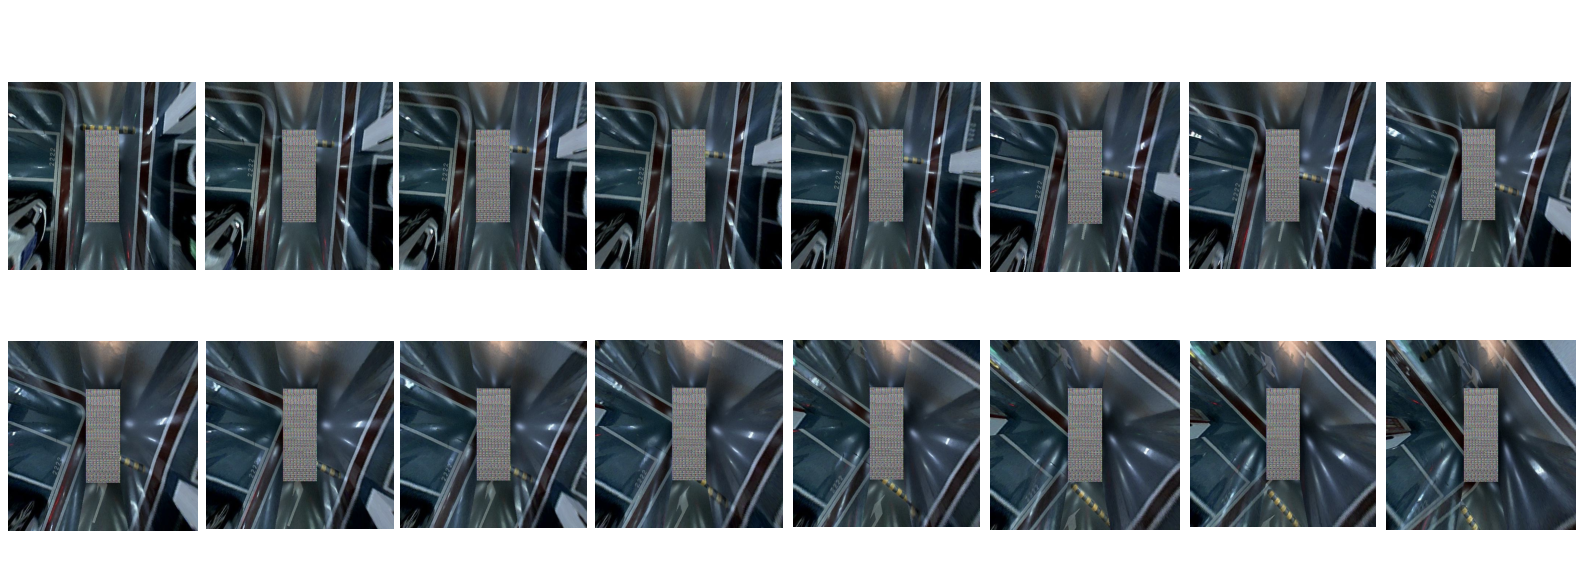
\includegraphics[width=1\textwidth]{figures/chp4/pstd.pdf}
\caption{PSTD数据集部分示例图片 \\Fig~\ref{fig_pstd}~Sample images from the PSTD dataset}
\label{fig_pstd}
\end{figure}

PSTD 数据集中的样本均由同一采集设备在短时间间隔内连续获取，相邻帧之间视角变化较小，停车位的空间结构整体保持一致，但在光照条件、局部遮挡、成像噪声及运动模糊等方面存在自然变化，能够较好地模拟真实自动泊车场景中的视频输入特性。如图\ref{fig_pstd}所示。在数据构建过程中，本文以当前帧作为监督目标帧，并选取其前一帧作为历史参考帧，形成二帧时序输入对：
\begin{equation}
(\mathbf{I}_{t-1}, \mathbf{I}_{t})
\end{equation}
其中仅对当前帧 $\mathbf{I}_{t}$ 使用原始 CRPS-D 数据集中的停车位关键点标注作为监督信号，从而避免跨帧标注不一致问题。

在保证标注精度与空间一致性的前提下，PSTD 数据集未对关键点坐标进行任何几何变换或插值处理，所有样本均直接继承 CRPS-D 的人工标注结果。同时，数据集中允许存在一定程度的帧间退化差异，以增强数据对复杂真实场景的代表性。

在实验设置中，PSTD 数据集共包含 8990 组连续帧样本，其中 7192 组用于训练，1798 组用于测试。训练集与测试集在场景类型、光照条件及停车位布局等方面保持一致分布，确保实验结果具有公平性与可比性。

通过构建 PSTD 时序数据集，本文在保留 CRPS-D 原有高复杂度与多样性的基础上，引入了明确的时间维度，为多帧时序特征融合方法的有效性验证提供了可靠的数据支撑。


\subsection{对比实验}
为验证所提出方法的有效性，本节在数据集PSTD上进行了充分的对比实验。
表 \ref{tab_pstc} 给出了本文方法与近期代表性停车位检测方法在 PSTD 时序数据集上的对比结果。由于现有停车位检测研究主要集中于单帧图像场景，当前该领域尚不存在公开可用的时序停车位检测数据集，因此本文仅能基于自构建的 PSTD 数据集开展时序对比实验。为保证对比的公平性与可复现性，本文选取具有公开实现的代表性方法，并在 PSTD 数据集上重新训练与测试其模型性能。

从实验结果可以看出，本文方法在查准率(Precision)、查全率(Recall)以及平均精度（AP）三项指标上均取得了最优表现。与基于图结构建模的 GCN 方法相比，本文方法在 AP 指标上提升了 +9.77\%，表明引入时序信息后，模型在复杂场景下对停车位结构的整体识别能力得到了显著增强。相较于 DMPR-PS 方法，本文方法在 查准率和查全率 上分别提升了 +0.96\% 和 +0.39\%，同时 AP 提升 +2.01\%，说明所提出的跨帧特征建模与动态时序融合策略能够在保持高召回率的同时，有效减少误检情况。

需要指出的是，尽管上述对比方法原本设计用于单帧停车位检测任务，但在 PSTD 数据集上的重新训练结果仍能够作为合理的对比基线，用于评估不同方法在连续帧场景下的检测性能。实验结果表明，单帧方法在面对帧间退化与遮挡时存在一定性能瓶颈，而本文提出的多帧时序停车位检测方法通过跨帧自注意力建模、动态结构感知融合以及时序鲁棒增强策略，能够更充分地利用时序上下文信息，从而在连续场景下取得更加稳定且准确的检测效果。

\begin{table}[!h]
\centering
\setlength{\tabcolsep}{8mm}
\caption{与开源SoTA方法对比\\
Table~\ref{tab_pstc}~Comparison with open-source SoTA methods}
\begin{tabular}{lccccc}
\toprule
    方法 &  Precision & Recall &  AP\\
\midrule
       GCN\cite{min2021attentional}  &  87.00\%	& 86.44\%	& 82.20\% \\
       DMPR-PS\cite{huang2019dmpr} &  91.57\%	& 91.94\%	& 89.96\% \\
       \textbf{Ours} &   \textbf{92.53\%} & \textbf{92.33\%} & \textbf{91.97\%}\\
\bottomrule
\end{tabular}
\label{tab_pstc}
\end{table}


\subsection{消融实验}

表 \ref{tab_3ab} 给出了本文所提出多帧时序停车位检测方法的消融实验结果。实验以单帧停车位检测模型作为基线，在此基础上逐步引入跨帧自注意力、动态时序融合以及时序鲁棒增强模块，以分析各个组成模块对整体检测性能的影响。

从实验结果可以看出，当仅使用单帧模型时，平均精度$AP$ 为 89.96\%。在此基础上引入跨帧自注意力模块后，模型性能提升至 91.46\%，取得了最为显著的性能增益。这一结果表明，通过显式建模相邻帧之间的特征关联关系，模型能够有效利用时序上下文信息，从而显著提升停车位结构的整体检测精度。

进一步加入动态时序融合模块后，$AP$ 提升至 91.71\%。该模块通过自适应调节当前帧与历史帧特征之间的融合权重，在抑制噪声干扰的同时增强结构一致性，从而在已有时序建模基础上进一步提升模型性能。

当三种时序相关模块全部引入后，模型取得了最高的 $AP$ 为 91.97\%。该结果验证了时序鲁棒增强策略在训练阶段对模型泛化能力的积极作用，使模型在面对光照变化、噪声干扰及局部遮挡等复杂情况时仍能保持稳定的检测表现。

综合消融实验结果可以看出，本文提出的跨帧自注意力、动态时序融合及时序鲁棒增强三种设计在性能提升方面具有良好的互补性，共同构成了一个有效且稳健的多帧时序停车位检测框架。


\begin{table*}[!h]
\centering
\setlength{\tabcolsep}{3mm}
\caption{消融实验结果 \\
Table~\ref{tab_3ab}~Results of ablation study}
\small
\begin{tabular}{ccccc}
\toprule
    Baseline(单帧) & 跨帧自注意力 & 动态时序融合  & 时序鲁棒增强 &  $AP$ \\
\midrule
    \checkmark  &  &  &  &  89.96\% \\
     \checkmark & \checkmark &  &  &  91.46\% \\
     \checkmark & \checkmark & \checkmark &  &  91.71\% \\
     \checkmark & \checkmark & \checkmark & \checkmark  & \textbf{91.97\%} \\
\bottomrule
\end{tabular}
\label{tab_3ab}
\end{table*}


\subsection{推理速度实验}

在推理效率方面，本文对比了所提出方法与两种代表性方法在 GPU 平台上的单帧推理时间，如表 \ref{tab_infer} 所示。DMPR 在 Nvidia Titan Xp 上的推理时间为 10 ms，表现出较高的推理效率；GCN 方法由于引入了图结构建模与复杂的节点关系推理，其单帧推理时间显著增加，达到 49 ms。相比之下，本文方法在 Nvidia 2080Ti 上的推理时间为 25 ms，整体处于合理区间。

尽管不同方法的测试平台存在一定差异，但从结果可以看出，本文方法在引入时序特征建模与结构感知机制的前提下，仍能够保持较为可控的推理开销。与基于图结构的 GCN 方法相比，本文方法显著降低了推理延迟；相较于纯单帧方法 DMPR-PS，推理时间有所增加，但换来了更强的时序一致性建模能力与整体检测性能提升。综合来看，本文方法在推理效率与检测精度之间取得了较为合理的平衡，具备在实际自动泊车场景中部署的潜力。

\begin{table}[!h]
\centering
\setlength{\tabcolsep}{10mm}
\caption{推理效率对比 \\
Table~\ref{tab_infer}~Comparison of inference efficiency}
\setlength{\tabcolsep}{10mm}
\begin{tabular}{lcc}
\toprule
   模型 & GPU型号 & 推理速度 \\
\midrule
    DMPR-PS\cite{huang2019dmpr} & Nvidia Titan Xp & 10ms \\
    GCN\cite{min2021attentional} & Nvidia Titan Xp & 49ms \\
    ours & Nvidia 2080Ti & 25ms \\
     
\bottomrule
\end{tabular}
\label{tab_infer}
\end{table}

此外，本文将训练好的模型部署至配备神经处理单元（Neural Processing Unit, NPU）的车规级处理器上，并在真实车辆平台上进行了在线推理测试。如图\ref{fig_intel}所示， 本文使用智能停车系统，将在 PSTD 数据集上训练的模型集成到该系统中。该系统在检测到可用停车位后，可以自动引导车辆进入停车位。实验结果表明，该模型在实际车载环境中能够稳定运行，推理帧率可达到约 \textbf{30 FPS}，验证了所提出方法在资源受限硬件条件下的实时性与工程可行性，能够满足低速自动泊车场景对感知算法的时序响应需求。


\begin{figure}[!h]
\centering
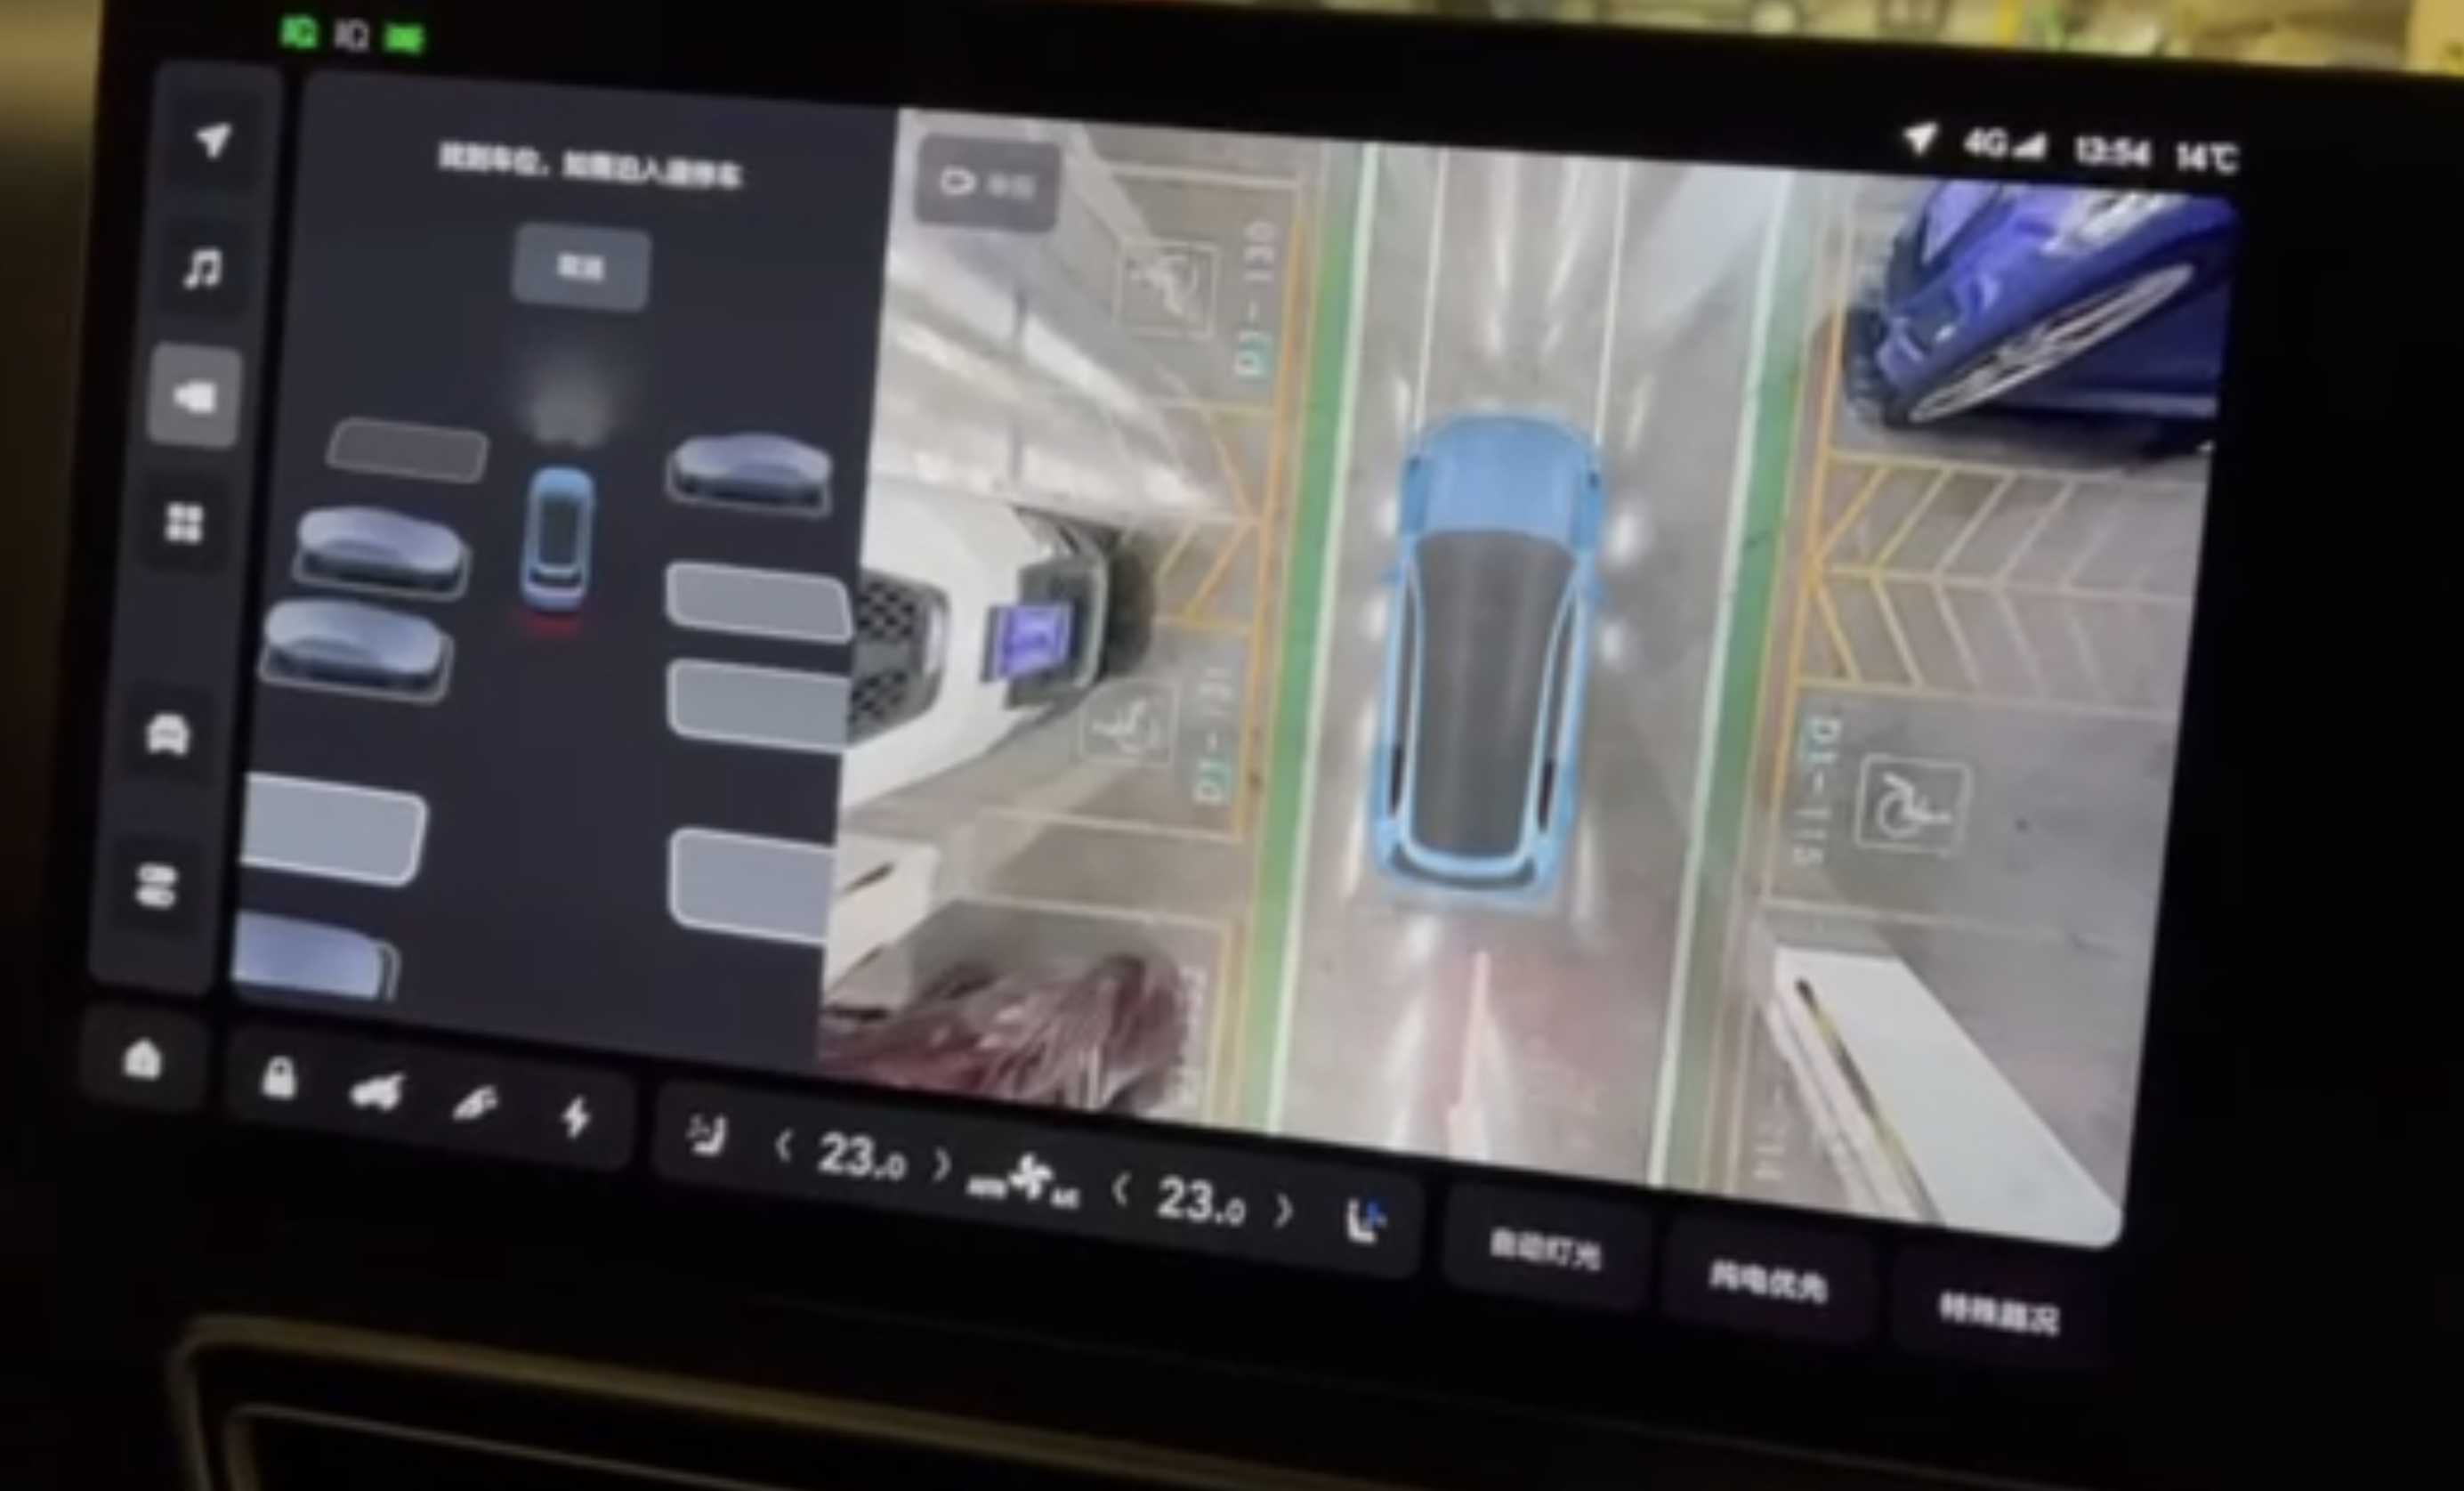
\includegraphics[width=1\textwidth]{figures/chp4/example.png}
\caption{智能停车系统 \\Fig~\ref{fig_intel}~Intelligent parking system}
\label{fig_intel}
\end{figure}


\section{本章小结}

在第二章单帧结构感知检测方法的基础上，本章进一步面向真实驾驶场景中连续帧输入条件下的检测稳定性问题，提出了一种多帧时序特征融合的停车位检测方法。该方法通过融合相邻帧之间的时序信息，有效缓解了单帧检测中由于瞬时遮挡、光照变化或视角抖动带来的不确定性。

首先，为充分利用连续帧之间的时序信息，提出了跨帧自注意力模块，通过显式建模当前帧与前一帧的空间特征关联关系，实现了跨帧信息的有效聚合。该模块能够增强模型在局部遮挡、光照变化及噪声干扰情况下对停车位结构的辨识能力，是时序建模的核心组成部分。

其次，提出了动态结构感知的时序融合模块，通过联合建模全局通道重要性与局部结构显著性，自适应地调节当前帧与历史帧特征的融合权重。这一设计能够在不同场景下合理平衡单帧信息与跨帧增强信息，进一步提高检测的稳定性与精度。

第三，为增强模型在复杂真实场景下的泛化能力，引入了时序鲁棒增强策略，在训练阶段对连续帧施加光度变化、噪声扰动、运动模糊及局部遮挡等增强操作，同时保持停车位关键点空间一致性。该策略使模型在面对帧间退化和环境扰动时仍能保持稳健性能。

在数据方面，本文基于 CRPS-D 构建了PSTD 时序数据集，为连续帧停车位检测提供了可靠的数据支撑，填补了该领域缺乏开源时序数据集的空白。通过系统的实验验证，包括对比实验和消融研究，结果表明本文方法在 Precision、Recall 以及 AP 指标上均优于现有方法，充分证明了跨帧建模、动态融合以及鲁棒增强三者的互补性与有效性。


总之，本章提出的方法在理论设计与实践验证上均显示出良好的性能，为多帧时序停车位检测提供了一种可行且高效的解决方案，同时为未来进一步研究连续场景下的智能交通感知任务奠定了基础。通过将停车位检测从单帧空间结构建模扩展至多帧时序建模，本章方法在保持端到端推理流程的同时，进一步提升了检测结果在时间维度上的一致性与鲁棒性，使所提出的停车位检测方法更加贴近实际应用场景。